\section{Introduction}
When studying intelligence, insects, reptiles, and humans have been found to possess neurons with the capacity to hold integers, real numbers, and perform arithmetic operations \cite{nieder-neuronal-number,rugani-arithmetic-chicks,gallistel-numbers-in-brain}.
In our quest to mimic intelligence we have put much faith in neural networks, which in turn has provided unparalleled and often superhuman performance in tasks requiring high cognitive abilities \cite{natureGo,googleNMT,resnet}.
However, when using neural networks to learn simple arithmetic problems, such as counting, multiplication, or comparison they systematically fail to extrapolate onto unseen ranges \cite{stillNotSystematic,suzgun2019evaluating,trask-nalu}. This can be a significant drawback when comparing in question answering \cite{naturalquestions} or counting objects in visual data \cite{johnson2017clevr,drewspaper}.

In this paper, we analyze and improve parts of the recently proposed Neural Arithmetic Logic Unit (NALU) \cite{trask-nalu}, which we will introduce in section \ref{sec:Nalu}. Our contributions are; an alternative formulation of the soft weight constraint with a clipped linear activation, parameter regularization that biases towards a sparse solution of $\{-1,0,1\}$, and a reformulation of the multiplication unit with a partial linearity. All of which significantly improves upon the existing $\text{NAC}_{+}$ and $\text{NAC}_{\bullet}$ units as shown through extensive testing on static arithmetic tasks.

The NALU is a neural network layer with two sub-units; the $\text{NAC}_{+}$ for addition/subtraction and the $\text{NAC}_{\bullet}$ for multiplication/division.
The sub-units are softly gated using a sigmoid function. The parameters, which are computed by a soft weight constraint using a tanh-sigmoid transformation, are learned by observing arithmetic input-output pairs and using backpropagation \cite{rumelhart1986learning}.
\begin{figure}[h]
\centering
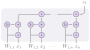
\includegraphics[scale=0.6]{graphics/nmu.pdf}
\caption{Visualization of NMU for a single output scalar $z_1$, this construction repeats for every element in the output vector $\mathbf{z}$.}
\end{figure}
We motivate our work by an investigation of the NALU components; the parameter transformation, the sub-units, $\text{NAC}_{+}$ and $\text{NAC}_{\bullet}$, and the soft gating mechanism.
The investigation uncovers the following analytical and empirical concerns; the gradients from the weight matrix construction in $\text{NAC}_{+}$ and $\text{NAC}_{\bullet}$ have zero expectation, the $\text{NAC}_{\bullet}$ has a treacherous optimization space with unwanted global minimas (as shown in figure \ref{fig:nac-mul-eps-issue}) and has exploding/vanishing gradients, when applying the $\text{NAC}_{+}$ in isolation, we observe that the wanted weight matrix values of $\{-1, 0, 1\}$ are rarely found, and our empirical results reveals that the NALU is significantly worse than hard-choosing either the $\text{NAC}_{+}$ or $\text{NAC}_{\bullet}$, indicating that the gating mechanism might not work as intended.

We avoid using gating as we see no obvious solution to simultaneously train two vastly different sub-units, the NAU/$\text{NAC}_{+}$ and NMU/$\text{NAC}_{\bullet}$, with a soft gating mechanism.
We will thus assume that the desired operation is already known, or can empirically be found by varying the network architecture.


\subsection{Learning a 10 parameter function}
Consider the static function $t = (x_1 + x_2) \cdot (x_1 + x_2 + x_3 + x_4)$ for $x \in \mathbb{R}^4$. To empirically validate the ability of $\mathrm{NAC}_{\bullet}$, NALU, and our proposed NMU we attempt to fit this function by only observing input-output pairs.

For the $\mathrm{NAC}_{\bullet}$, NALU, and NMU we conduct 100 experiments with different seeds and stop after $2 \cdot 10^5$ iterations. The results in table \ref{tab:very-simple-function-results} show that NMU has a higher success rate and converges faster.
%When inspecting the $6\%$ that did not converge, we found the issue to be underflow when $w = 0$ in the multiplication layer.
\begin{table}[!h]

\caption{\label{tab:very-simple-function-results}Comparison of the success-rate, when the model converged, and the sparsity error for all weight matrices, with 95\% confidence interval on the $t = (x_1 + x_2) \cdot (x_1 + x_2 + x_3 + x_4)$ task. Each value is a summary of 100 different seeds.}
\centering
\begin{tabular}{crllll}
\toprule
\multicolumn{1}{c}{Op} & \multicolumn{1}{c}{Model} & \multicolumn{1}{c}{Success} & \multicolumn{2}{c}{Solved at} & \multicolumn{1}{c}{Sparsity error} \\
\cmidrule(l{3pt}r{3pt}){1-1} \cmidrule(l{3pt}r{3pt}){2-2} \cmidrule(l{3pt}r{3pt}){3-3} \cmidrule(l{3pt}r{3pt}){4-5} \cmidrule(l{3pt}r{3pt}){6-6}
 &  & Rate & Median & Mean & Mean\\
\midrule
 & $\mathrm{NAC}_{\bullet}$ & $13\% {~}^{+8\%}_{-5\%}$ & $5.5 \cdot 10^{4}$ & $5.9 \cdot 10^{4} {~}^{+7.8 \cdot 10^{3}}_{-6.6 \cdot 10^{3}}$ & $7.5 \cdot 10^{-6} {~}^{+2.0 \cdot 10^{-6}}_{-2.0 \cdot 10^{-6}}$\\

\nopagebreak
 & NALU & $26\% {~}^{+9\%}_{-8\%}$ & $7.0 \cdot 10^{4}$ & $7.8 \cdot 10^{4} {~}^{+6.2 \cdot 10^{3}}_{-8.6 \cdot 10^{3}}$ & $9.2 \cdot 10^{-6} {~}^{+1.7 \cdot 10^{-6}}_{-1.7 \cdot 10^{-6}}$\\

\nopagebreak
\multirow{-3}{*}{\centering\arraybackslash $\bm{\times}$} & NMU & $\mathbf{94\%} {~}^{+3\%}_{-6\%}$ & $\mathbf{1.4 \cdot 10^{4}}$ & $\mathbf{1.4 \cdot 10^{4}} {~}^{+2.2 \cdot 10^{2}}_{-2.1 \cdot 10^{2}}$ & $\mathbf{2.6 \cdot 10^{-8}} {~}^{+6.4 \cdot 10^{-9}}_{-6.4 \cdot 10^{-9}}$\\
\bottomrule
\end{tabular}
\end{table}

